\section{Investigation/Research}

In this section we describe our investigation and research over the proposal readings. Investigation throughout the examination of the reading facts, novel possibilities and results. Also, addressing the research reasoned conclusions of those readings.

\subsection{Interaction Methods}

The impact of Interactive Machine Learning (iML) for the Biomedical development as a system recognition using Human-In-The-Loop (HITL) approach is being demonstrated by Yimam et al. \cite{yimam2015interactive} in a paper titled as \textit{Interactive and Iterative Annotation for Biomedical Entity Recognition}. The authors demonstrate that during text annotations (Figure \ref{fig:webanno}), for instance in several medical images, a Machine Learning (ML) model is built on previous text annotations, while being used to propose labels (semantic over medical imaging) for subsequent of text annotations. Such interactions are improving the development of quality dataset of text annotations.

\hfill

\begin{figure}[h]
\center
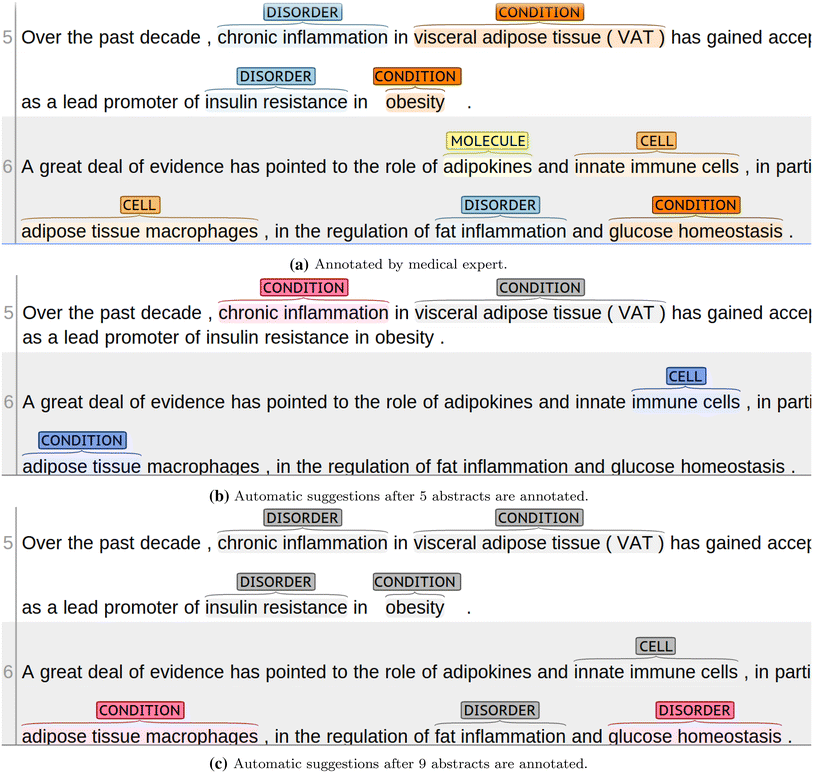
\includegraphics[width=0.50\textwidth]{webanno.png}
\caption{WebAnno Automation Suggestions}
\label{fig:webanno}
\end{figure}

\hfill

\clearpage

The authors conducted two experiments. For the first experiment, the authors carry out an iterative text annotations for an experimental simulation and showed that only a handful of medical abstracts are needed to be annotated, producing suggestions that are increasing the text annotation speed. For the second experiment, clinicians have conducted a case study in medical terms documentation annotations for their research. The experiments validated the authors' method in terms of qualitative and quantitative analysis, rising a more personalised, responsive information extraction by the use of technology.

To better explain the experiment we further detail it. Once a first round of text annotations is completed, WebAnno \cite{yimam2013webanno} starts automatically by ordering the provided initial suggestions. In Figure \ref{fig:webanno}, the automation component is suggesting immediately the entity of text annotations after the first round. By using the suggestion, the clinician continues annotating. After several annotated abstracts, the quality and quantity of suggestions have been increased.

This work might be important to us since the authors investigated the impact of adaptive ML for text annotations. This sentence can also be applied to our medical imaging annotations. Or at least, we hope so. The authors tackle medical entity recognition on texts from several abstracts. From their work, we can identify the need of imaging tagging for applications such as DICOM meta-information extraction \cite{vizza2016annotation}, imaging exploring and patient history extraction \cite{han2015texture} and identifying the medical imaging annotation acquisition bottleneck which is specially severe on the medical domain. Also, the authors carried out two different experiments showing us the utility of a HITL approach for suggesting annotations in order to speed up the process and thus to widen the bottleneck.

\subsection{Recommender Systems}

Titled as \textit{Each to His Own: How Different Users Call for Different Interaction Methods in Recommender Systems}, the work done by Knijnenburg et al. \cite{knijnenburg2011each} compares five different ways of interacting with an attribute-based recommender system. It show us that different types of users prefer different interaction methods. Therefore we need to take into consideration their conclusions to manage if we would like to give clinicians more then one interaction technique depending on their user profile.

In their experiment with a recommender system the interaction methods are compared in terms of perceived control, understandability, trust in the system, satisfaction and system effectiveness. All characteristics from this study are important to us to measure also. The results showed us that most of the domain experts, like our clinicians, are most satisfied with a hybrid recommender that combines implicit and explicit elicitations. On the other hand, novices and maximisers seem to benefit more from a non-personalised recommender that just displays the most popular outputs for the user.

Since we are aim to give annotation recommendations on the medical images displayed in our system, we are interested in their work since they study the combination between an implicit and explicit elicitation, also potentially adequate to our annotation recommender. Their work is also important, since the authors have shown that the best interaction method for a recommender system depends on the characteristics of the users, showing us how to profile those characteristics and how to measure it, while doing several conclusions over the user study. Those analysis and conclusions are of chief importance to us and, despite of having some drawbacks, a careful consideration of a clinician characteristics in the design and evaluation of these methods can lead to significantly better systems.














